\section{Analysis}
\subsection{Identifying the Fe-57 transition peak}
\begin{figure}[H]
\centering
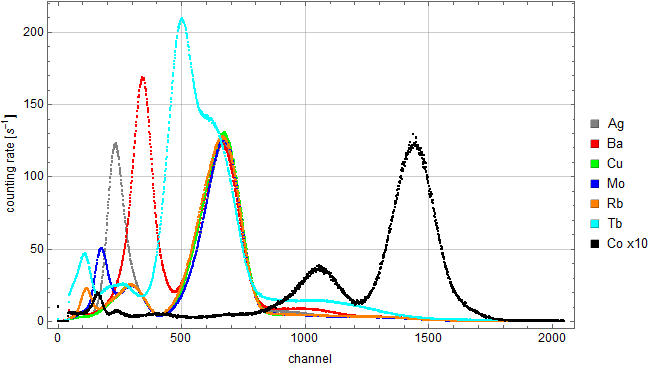
\includegraphics[width=1\linewidth]{../results/calibration/spectra}
\caption[Reference spectra]{Plot of all recorded reference spectra and the cobalt source (upscaled by factor 10 for better comparability)}
\label{fig:analysis:spectra}
\end{figure}
Around channel 700 all target samples have clearly defined peak. For Terbium(Tb) this peaks blends with its $K$-line. That peak is caused by photons of the americium source, passing through the targets without interacting. The $K_\alpha$-line of copper (Cu) is beyond the left edge and therefore not meassured. The peak positions are estimated from the fig \ref{fig:analysis:spectra}. The error is estimated to be $s_{Ch}=10$. The Result can be seen in table \ref{tb:analysis:peakpos}. One can already identify the peak since it has to lie between the Rb-peak and the Mo-peak, which is suggesting that the peak furthest to the left (around channel 160) belongs to the \unit{14.4}{keV} line.

\begin{table}[H]\centering
	\begin{tabular}{@{}llllll@{}}
		\toprule
		 traget & energy [keV]& peak channel  \\
		\midrule
		Cu & 8.04 & - \\
		Rb & 13.37 & 120 \\
		Mo & 17.44 & 180 \\
		Ag & 22.10 & 230 \\
		Ba & 32.06 & 340 \\
		Tb & 44.23 & 500\\
		\bottomrule
	\end{tabular}
	\caption[peak positions]{number of the channel for the $K$-line peaks}
	\label{tb:analysis:peakpos}
\end{table}

The Linear function $E(ch)=a\cdot ch+b$ was fitted to the data see figure
\begin{figure}[H]
\centering
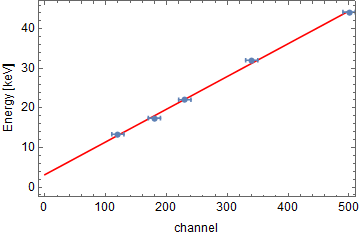
\includegraphics[width=1.0\linewidth]{../results/calibration/fit}
\caption[MCA calibration]{Linear fit for the calibration of the MCA}
\label{fig:calibrationfit}
\end{figure}
The results are:
\begin{equation}
\begin{aligned}
	a &= (0.083\pm0.002)keV\\
	b &= (3.2 \pm 0.6)keV
\end{aligned}
\end{equation}
The position of the 14.4keV peak should be at\footnote{error calculated according to gaussian error propagation. Unless specified otherwise, all errors of values calculated with other values are determined this way}:
\begin{equation}
ch_{14.4keV}=\frac{14.4keV-b}{a}=135\pm4
\end{equation}
A Comparison with figure \ref{fig:analysis:spectra} shows that the peak furthest to left is the closest ($ch=160\pm10$)to this value, however the values lie more almost two standard deviations apart. Fortunately, an exact calibration is not needed for further analysis.
\subsection{Compton}
High energy photons such as those from the transitions with \unit{122}{keV} and \unit{136}{keV} lose energy when passing through matter via the Compton effect. Some of these photons will randomly fall within the energy windows that was set for the measurements and thus pose an underground that needs to be subtracted from the data for parts of the further analysis. Since higher energy photons lose their energy slower than lower energy photons when passing through matter, one can separate the two by placing aluminum plates in the beam with a range of thicknesses. The count rate decreases exponentially with the thickness $d$ 
\begin{equation}
\dot{N}=\dot{N}_0e^{-\mu d}
\end{equation}
measurements were taken for absorber thicknesses between $d=\unit{0.21}{mm}$ and $d=\unit{12.43}{mm}$, which were measured with a caliper to such high precision that the error is far smaller than the Poisson error on the count rates and is thus neglected. Figure \ref{fig:comptonbackground} shows the measured data.
\begin{figure}
\centering
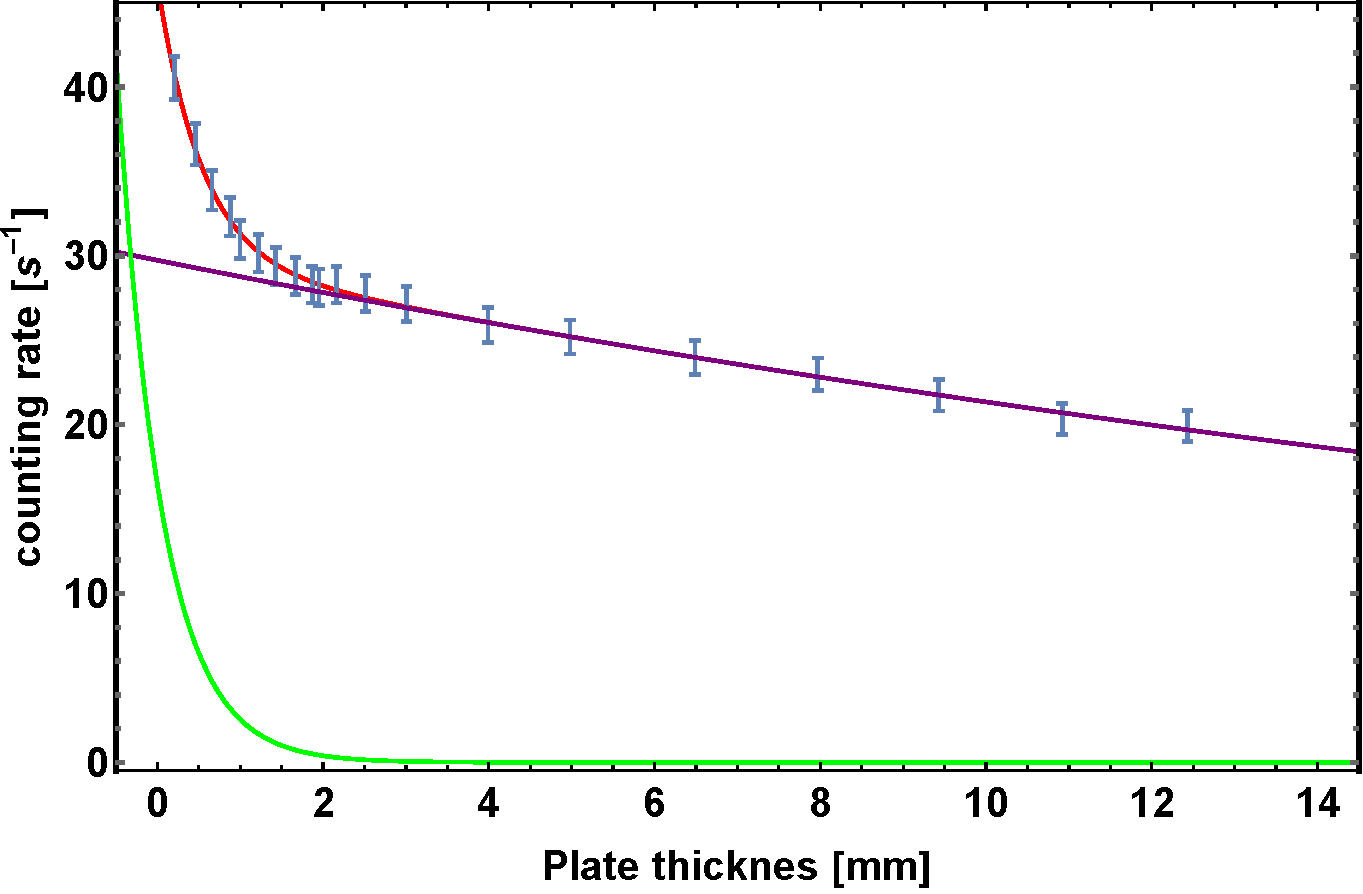
\includegraphics[width=1.0\linewidth]{graphics/comptonbackground}
\caption[Compton background data]{The compton background data along with the fitted sum of the two exponential functions in red. The curve for Compton underground is colored purple and that for the \unit{14,4}{keV} photons green.}
\label{fig:comptonbackground}
\end{figure}
As two processes with different speeds, $\mu_{C}$ of the Compton background and $\mu_0$ of the actual data, are expected, the fit function for the count rates for varying absorbers is
\begin{equation}
\dot{N}(d)=A_C\cdot e^{-\mu_C d}+A_0\cdot e^{-\mu_0 d}
\end{equation}
The resulting fit parameters for the Compton underground were
\begin{align}
A_C&=\unit{(29.74\pm0.17)}{s^{-1}}\\
\mu_C&=\unit{(0.0331\pm0.0009)}{mm^{-1}}
\end{align}
As no aluminum plates are used during regular measurements, the value for $d=0$, and thus the fit parameter $A_C$, is the underground rate to be deducted from future measurements.

\subsection{Attenuation of the acrylic glass}
The acrylic glass in which the sample is cased absorbs some of the radiation. To quantify this, a plate of acrylic glass of roughly the same thickness as the one used to case the sample can be but into the beam. One measurement is taken with the plate and one without. The thickness of the plate was measured as $d=\unit{(1.94\pm0.01)}{mm}$. The resulting count rates were
\begin{align}
\dot{N}_0&=\unit{(107.4\pm0.3)}{s^{-1}}\\
\dot{N}_A&=\unit{(84.8\pm0.3)}{s^{-1}}
\end{align}
where the uncertainties stem from the Poisson errors on the number of counts. With the values given for the attenuation coefficient $\mu/\rho=\unit{1.101}{cm^2/g}$ and the density of the acrylic glass $\rho=\unit{1.19}{g/cm^3}$ in \cite{anleitung}, the mass attenuation coefficient $\mu=\unit{1.31019}{1/cm}$ can be calculated. With this value as well as the thickness of the plate, the count rate after the acrylic glass can also directly be calculated from the count rate without the acrylic glass as
\begin{equation}
\dot{N}_A^{calc}=\dot{N}_0\cdot e^{-\mu d}=\unit{(83.3\pm0.3)}{s^{-1}}
\end{equation}
The two values agree only with their $2\sigma$ intervals. The literature value $\mu/\rho=\unit{1.101}{cm^2/g}$ is actually listed for energies of $E_\gamma=\unit{15}{keV}$, which is slightly more than the that of the $\unit{14.4}{keV}$ transition. However, the value is higher for lower energies, which means that using a value for the exact energies of the photons in this experiment would lead to an even lower calculated count rate. The likely cause for the disagreement of the values is thus likely that the thicknesses of the plates do no match. A quick calculation reveals that a disagreement of 5\% would bridge the gap and have the values agree within their $1\sigma$ intervals.
\subsection{Single line absorber}
The results for the measurement of the absorption spectrum of stainless steel can be seen in figure \ref{fig:single line absorber:fitresult}. To evaluate the data a voigt function (convolution of a Gaussian and Lorentz) was fitted to it:
\begin{equation}
f(v)=B- A \cdot Voigt((v-v_0),\delta,\sigma )
\end{equation}
where $v$ is the absorber velocity, $v_0$ the peak position, $\delta$ is the 
\begin{figure}[H]
\centering
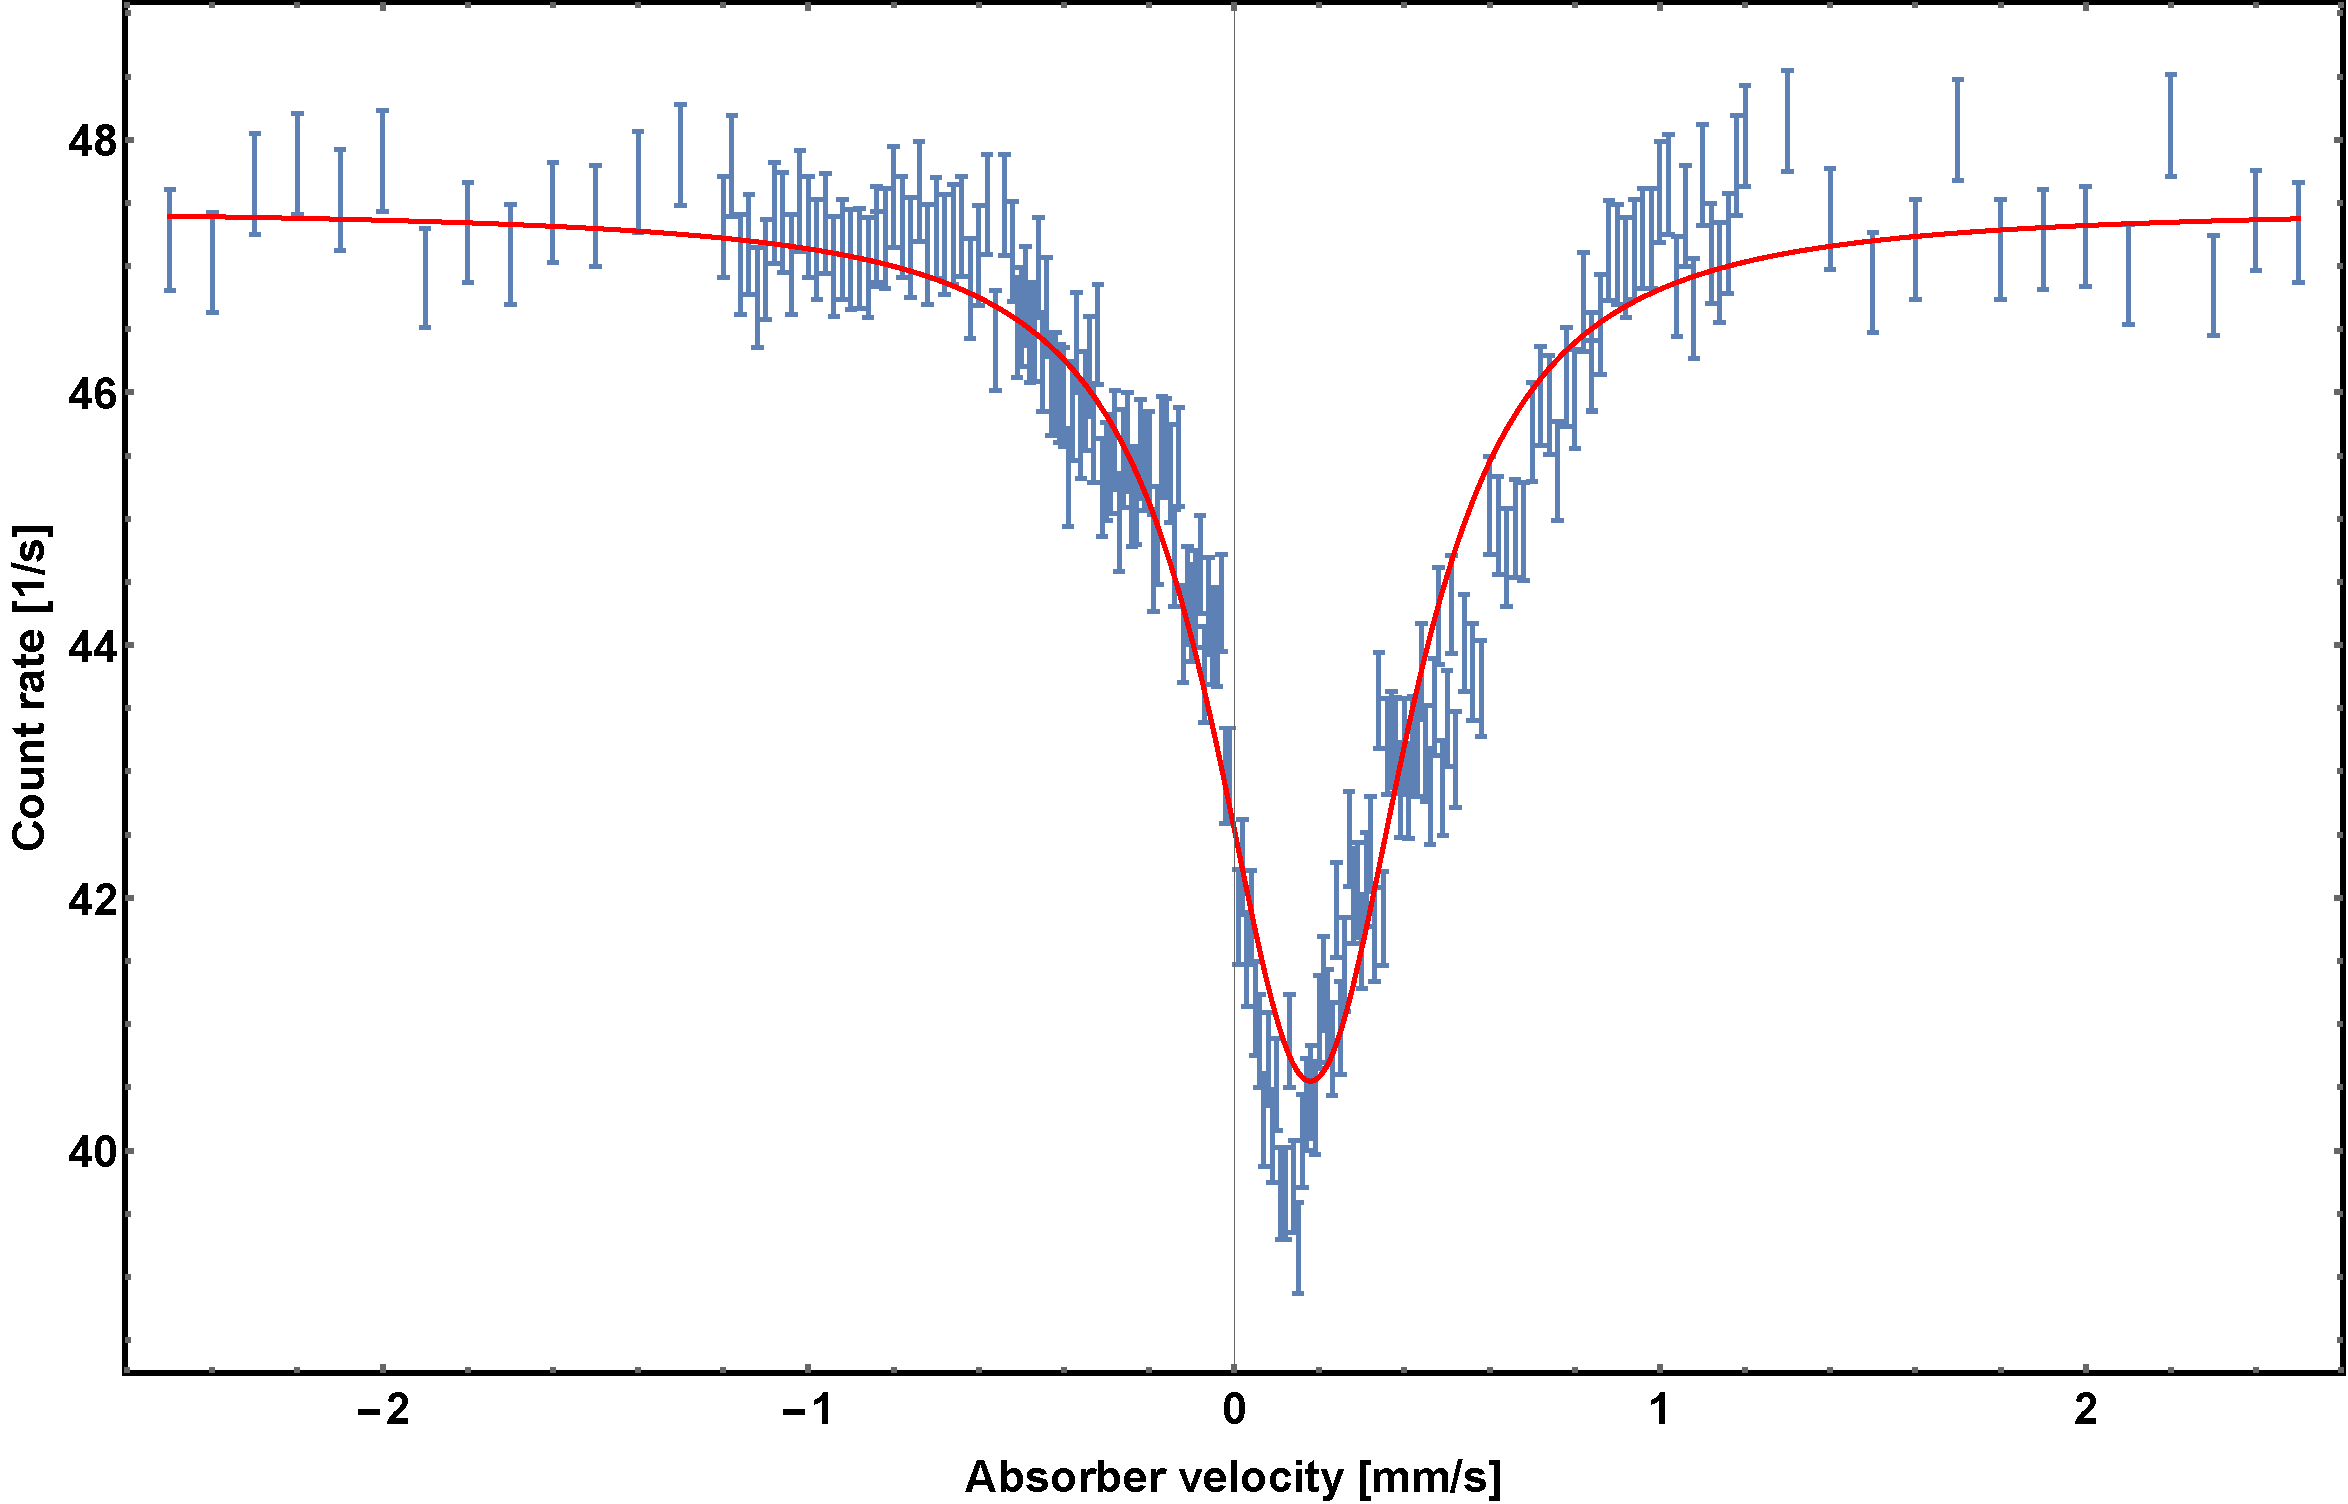
\includegraphics[width=1.0\linewidth]{../results/steel/voigtfittry.pdf}
\caption[Stainless steel spectrum]{Measured absorption spectrum for stainless steel and Voigt fit.}
\label{fig:single line absorber:fitresult}
\end{figure}
The fit results are:\\ \ \\
$\begin{array}{l|llll}
\text{} & \text{Estimate} & \text{Standard Error} \\
\hline
v_0 & 0.179 & 0.005\\
\sigma  & 0.25 & 0.03 \\
\delta  & 0.14 & 0.10\\
\text{B} & 47.46 & 0.11\\
A & 5.8 & 0.4 &\\
\end{array}$
The fit function exhibits notable differences from the data. The data peak lies about $unit{0.05}{mm/s}$ closer to zero than the Voigt peak and there is a noticeable asymmetry. The left flank is steeper than the right. This is a hint that the model does not reflect the data fully.
\subsubsection{Isomeric shift} \ \\
Since the background is constant it only effects variable $B$ of the fit function, therefore
with the parameter $v_0$ one can calculate the isomeric shift, without having to correct for the background. \ref{eq:diffdopplershift}:
\begin{equation}
E_{iso} = (8.61\pm0.24)\cdot 10^{-9} eV
\end{equation}
\subsubsection{Effective absorber thickness}
\label{sec:effab}
 \ \\
The effective absorber thickness is given by \cite{anleitung}:
\begin{equation}
T_A = f_An_A\beta\sigma_0d_A
\label{eq:effective absorber thickness}
\end{equation}
where $d_A = 25\mu m$ is the absorber thickness, $n_A$ is the number of iron atoms per volume, $\beta=0.022$ the ratio of Fe-57 in the isotope mixture, $\sigma_0$ the cross section and $f_A=0.8$ the Debye-Waller-factor of the absorber.
To calculate $n_A$ literature values are used (\cite{webelements}):

\begin{equation*}
\begin{aligned}
N_A &= 6.022 \cdot 10^{23} mol^{-1} \qquad& \text{Avogadro constant}\\
\rho_{Fe} &= 7.874 g/cm^3 \qquad& \text{density of iron} \\
A_Fe &= 55.845 g/mol \qquad& \text{molar mass of iron}\\
r &=  (0.70\pm0.05) \qquad& \text{fraction of iron in the absorber\cite{anleitung}}
\end{aligned}
\end{equation*}
The number of Fe atoms per volume is then given by:
\begin{equation*}
\frac{\rho_{Fe}}{A_Fe}N_A\cdot r= (5.9\pm0.4)\cdot 10^{22} cm^{-3}
\end{equation*}
The absorption cross section is given by \cite{Wegener}:
\begin{equation}
\sigma_0= \frac{\lambda^2}{2\pi} \left(\frac{2I^*+1}{2I+1}\right) \frac{1}{1+\alpha}
\end{equation}
where $\alpha =9$ (see \cite{Wegener}) is the conversion coefficient, $\lambda$ the wavelength of the absorbed photon, $I^*=3/2$ and $I=1/2$  are the nuclear spins of the excited and ground state. With $\lambda = \frac{hc}{E_\gamma}=86.14 pm$, the cross section is:
\begin{equation}
\sigma_0=2.36\cdot 10^-22m^2
\end{equation}
Plugging those values in equation \ref{eq:effective absorber thickness}, the effective absorber thickness is:
\begin{equation}
T_A = (6.2\pm 0.4)
\end{equation}
\subsubsection{Debye Waller factor of the source}
The Debye-Waller-factor is related to the count rate with no absorption $Z(\infty)$, the minimal count rate $Z(v_min)$ (maximal absorption) and the effective absorber thickness $T_A$ \cite{Wegener}:
\begin{equation}
\frac{Z(\infty)-Z(v_{min})}{Z(\infty)}=f\cdot [1-exp(-\frac{T_A}{2})J_0(\frac{iT_A}{2})]
\label{eq:debye}
\end{equation}
$i$ is the imaginary unit and $J_0$ the order zero Bessel function. The count rates on the left can be determined from the fit function $f(v)$ and the Compton background $A_C$:
\begin{equation}
\begin{aligned}
Z(\infty) &= B - A_C\\
Z(v_{min}) &= A-A_C\\
\end{aligned}
\end{equation}
Rearranging equation \ref{eq:debye} we get for the Debye-Waller factor of the source
\begin{equation}
f_s= 0.51\pm0.08
\end{equation}
The rather big error ($15\%$) is mainly caused by the uncertainty of $Z(v_{min})$ since all errors of the fit function parameters contribute.

\subsubsection{Life time of the 14.4keV state}
\paragraph{From the fit}\ \\
From the Voigt fit the half width $\delta = 0.14 \pm 0.10$ of the convoluted Lorentzian can be extracted. It has to be noted, that $\delta$ from the fit is still in units of velocity (mm/s), so using equation \ref{eq:diffdopplershift} the wanted half width $\Gamma$ is:
\begin{equation}
\Gamma  = \unit{6.2\pm4.6\cdot 10^{-8}}{eV}
\end{equation}
With Heisenberg's uncertainty relation $\Gamma \cdot \scalebox{1.5}{$\tau$}=\hbar$, the mean life time is:
\begin{equation}
\scalebox{1.5}{$\tau$}= (11\pm8)ns
\end{equation}
The fit uncertainty propagates through the calculation and is responsible for the 
relative error of over $70\%$. Despite of this the literature value \scalebox{1.5}{$\tau$}$_{lit}$=141ns is still more than seven standard deviations away from the determined value.

\paragraph{From the effective absorber thickness} \ \\
The relative line broadening $\Gamma_a/2\Gamma$ is determined graphically from figure \ref{fig:absorberthicknessevaluated}. For this purpose the program Inkscape was used. By measuring the length of each coordinate axes in pixels, factors are determined, allowing the conversion between line lengths in pixels and their corresponding values.\\
\begin{figure}[hbp]
	\centering
	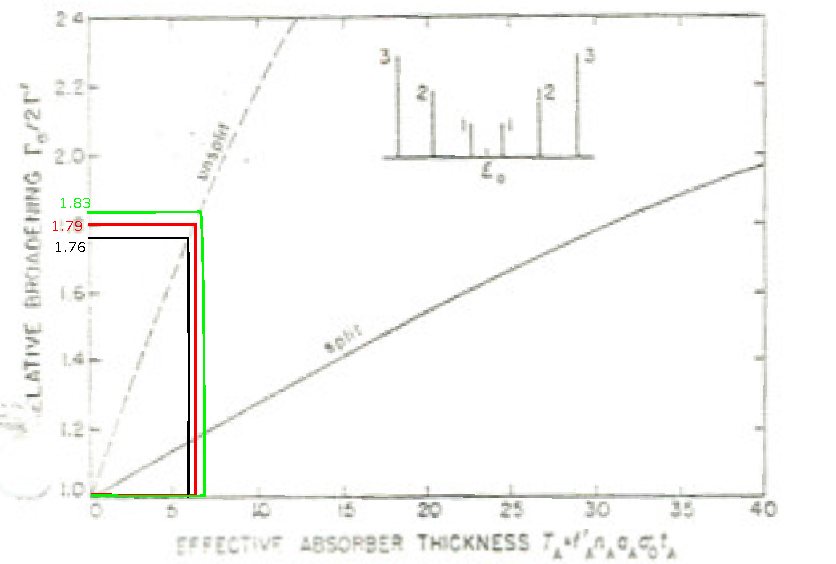
\includegraphics[width=1.0\linewidth]{graphics/absorberthicknessevaluated}
	\caption{Graphical determination of the relative line broadening\cite{Frauenfelder}}
	\label{fig:absorberthicknessevaluated}
\end{figure}
The effective absorber thickness was calculated in section \ref{sec:effab}. To estimate the error, the relative broadening was also determined for $T_A\pm s_{T_A}$. The results are:
\begin{table}[H]\centering
	\begin{tabular}{@{}llllll@{}}
		\toprule
		$T_A$ & $\frac{\Gamma_a}{2\Gamma}$ \\
		\midrule
		5.8 & 1.76\\
		6.2 & 1.79 \\
		6.6 & 1.83 \\
	\end{tabular}
	\caption[relative broadening]{relative broadening for different absorber thicknesses}
	\label{tb:relative broadening}
\end{table}
For the error estimation the bigger difference (0.04) is chosen. As the peak width of the absorber, the width of the fitted Voigt profile is used, calculated with an empirical  approximation($0.02\%$ accuracy)\cite{Olivero}:
\begin{equation}
\Gamma_a=0.5\cdot (1.0692\cdot \delta+\sqrt{0.86639\cdot \delta^2 + 4\cdot (2\sigma\sqrt{2ln(2)})})
\end{equation}
and with the values from the Voigt fit for $\delta$ and $\sigma$
\begin{equation}
\Gamma_a=\unit{(32\pm4)}{neV}
\end{equation}
and
\begin{equation}
\Gamma=\unit{(8.9\pm0.6)}{neV}
\end{equation}
Due to the time-energy uncertainty the mean life time is then given by:
\begin{equation}
\scalebox{1.5}{$\tau$}=\hbar/\Gamma=\unit{(6.5\pm0.4)}{ns}
\end{equation}